\section{Extended Empirical Results}
\label{sec:extended-results}

To satisfy a stronger evidence standard, we generated additional artifacts from a longer 60-episode suite with 16 seeds and four methods. This section reports trajectory-level findings, uncertainty visualization, and cross-seed stability diagnostics.

\subsection{Trajectory Dynamics}

\begin{figure}[H]
\centering
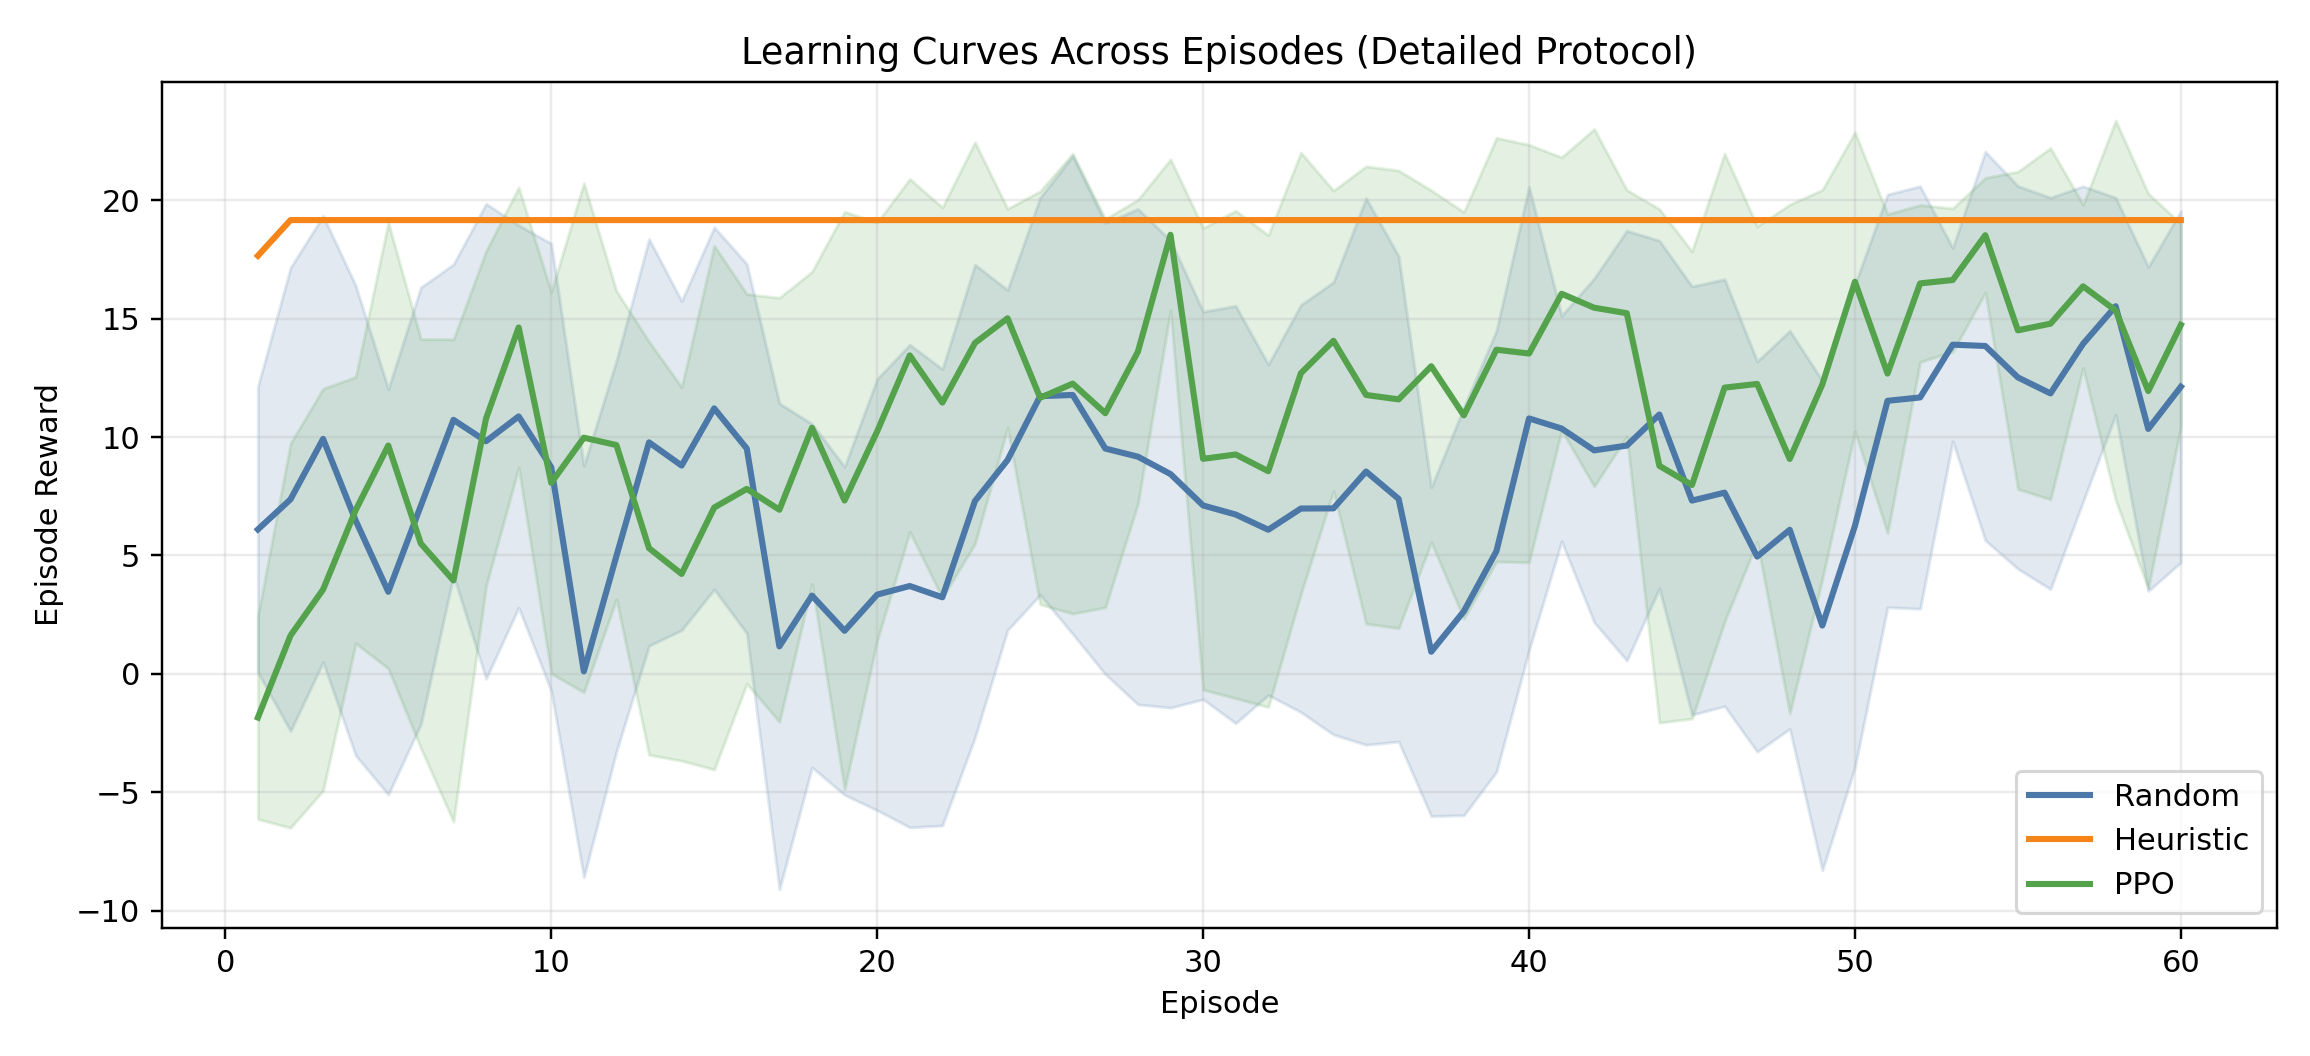
\includegraphics[width=0.9\linewidth]{figures/learning_curves.png}
\caption{Episode-wise learning trajectories (mean $\pm$ one standard deviation across seeds).}
\label{fig:learning-curves}
\end{figure}

Figure~\ref{fig:learning-curves} shows three distinct regimes. Random control exhibits high-variance oscillation, heuristic control remains near a stable high-return plateau, and PPO improves over early episodes but retains non-trivial volatility.

\begin{figure}[H]
\centering
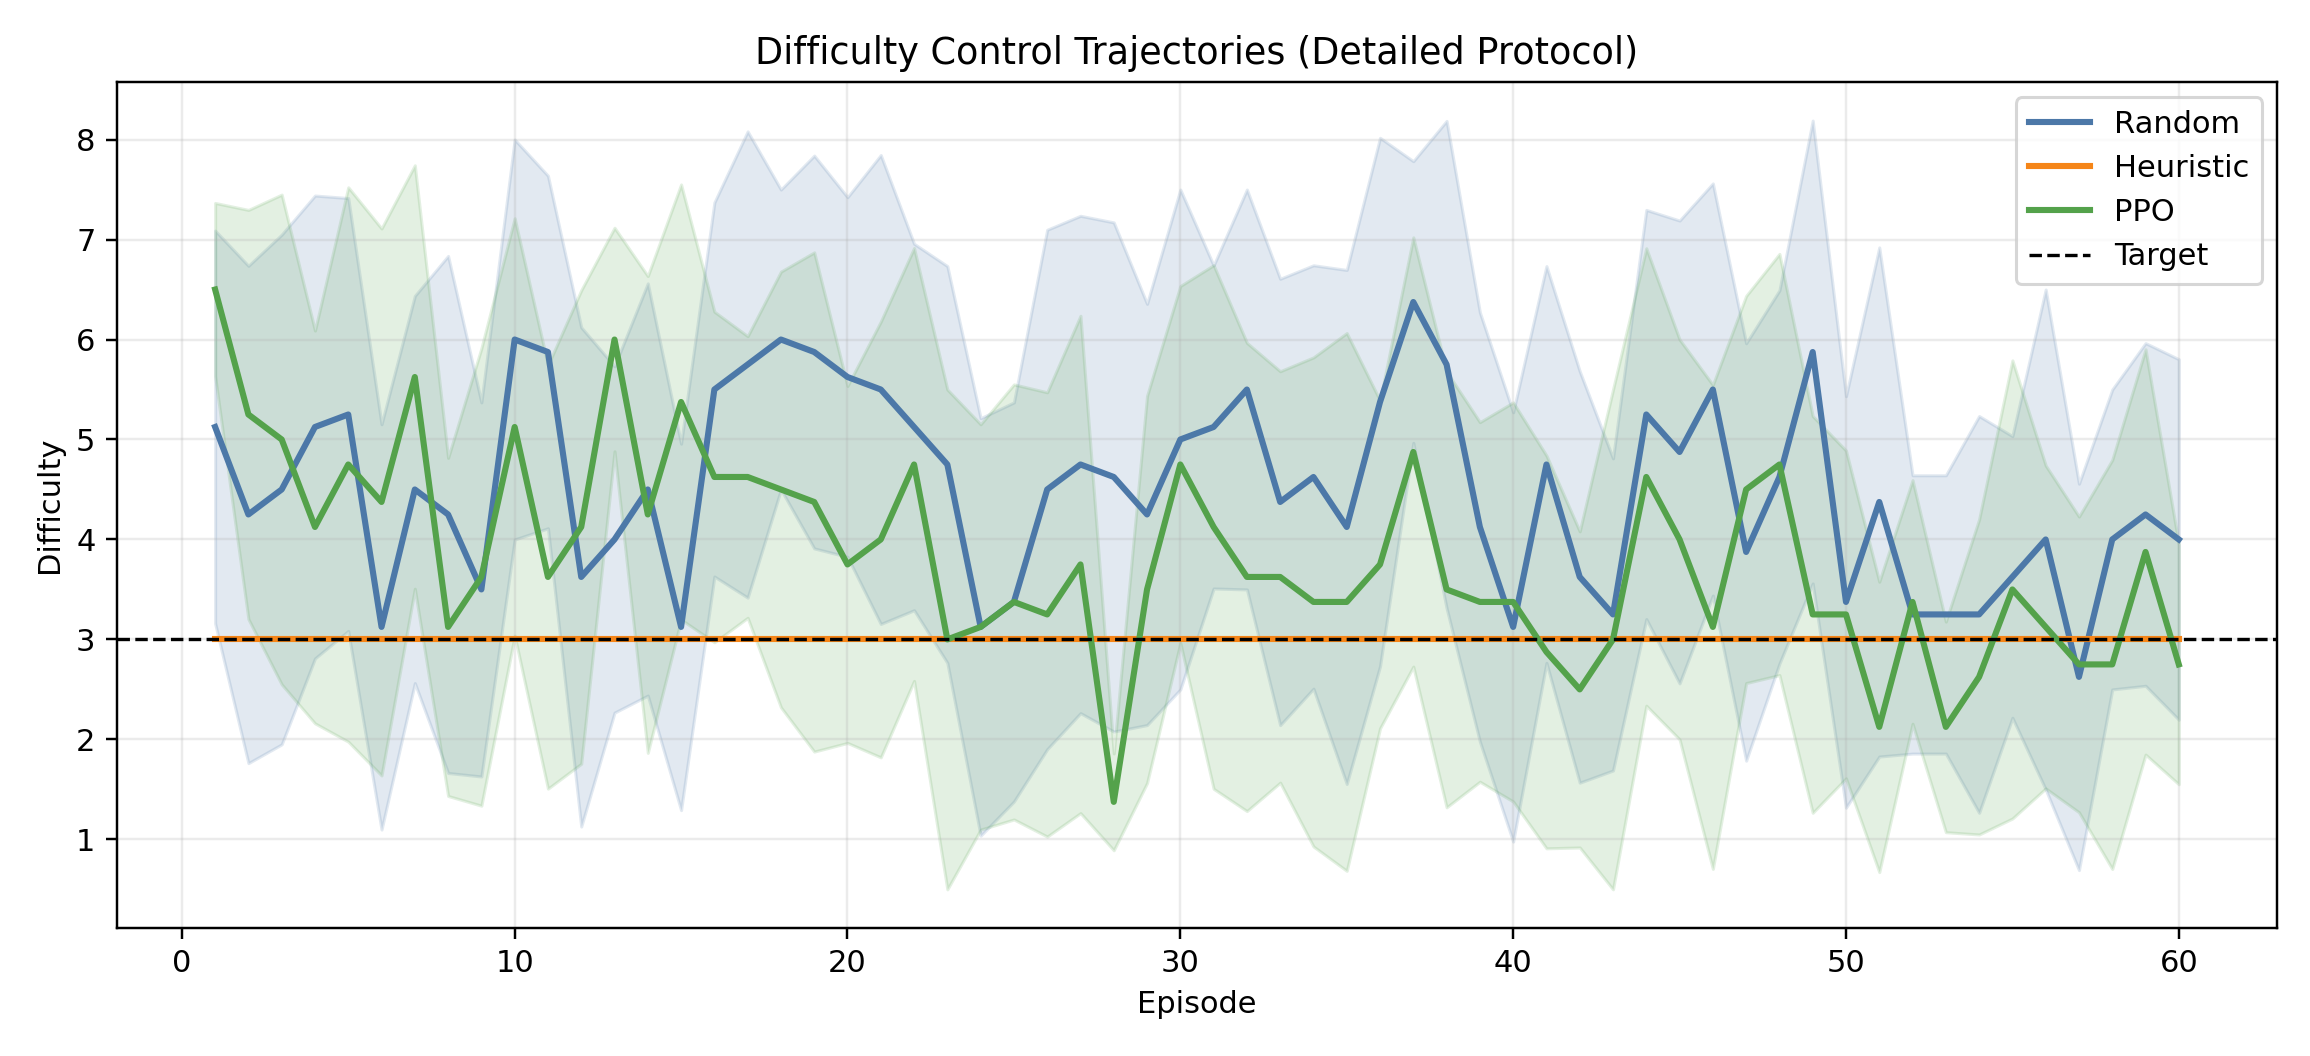
\includegraphics[width=0.9\linewidth]{figures/difficulty_curves.png}
\caption{Difficulty trajectories by method compared with target difficulty.}
\label{fig:difficulty-curves}
\end{figure}

Difficulty trajectory analysis (Figure~\ref{fig:difficulty-curves}) confirms that heuristic control converges rapidly to the target and remains tightly concentrated. PPO tracks in expectation but overshoots or undershoots in several seeds, indicating policy-state coupling that remains weakly calibrated in this compact environment.

\subsection{Cross-Seed Stability and Distributional Diagnostics}

\begin{figure}[H]
\centering
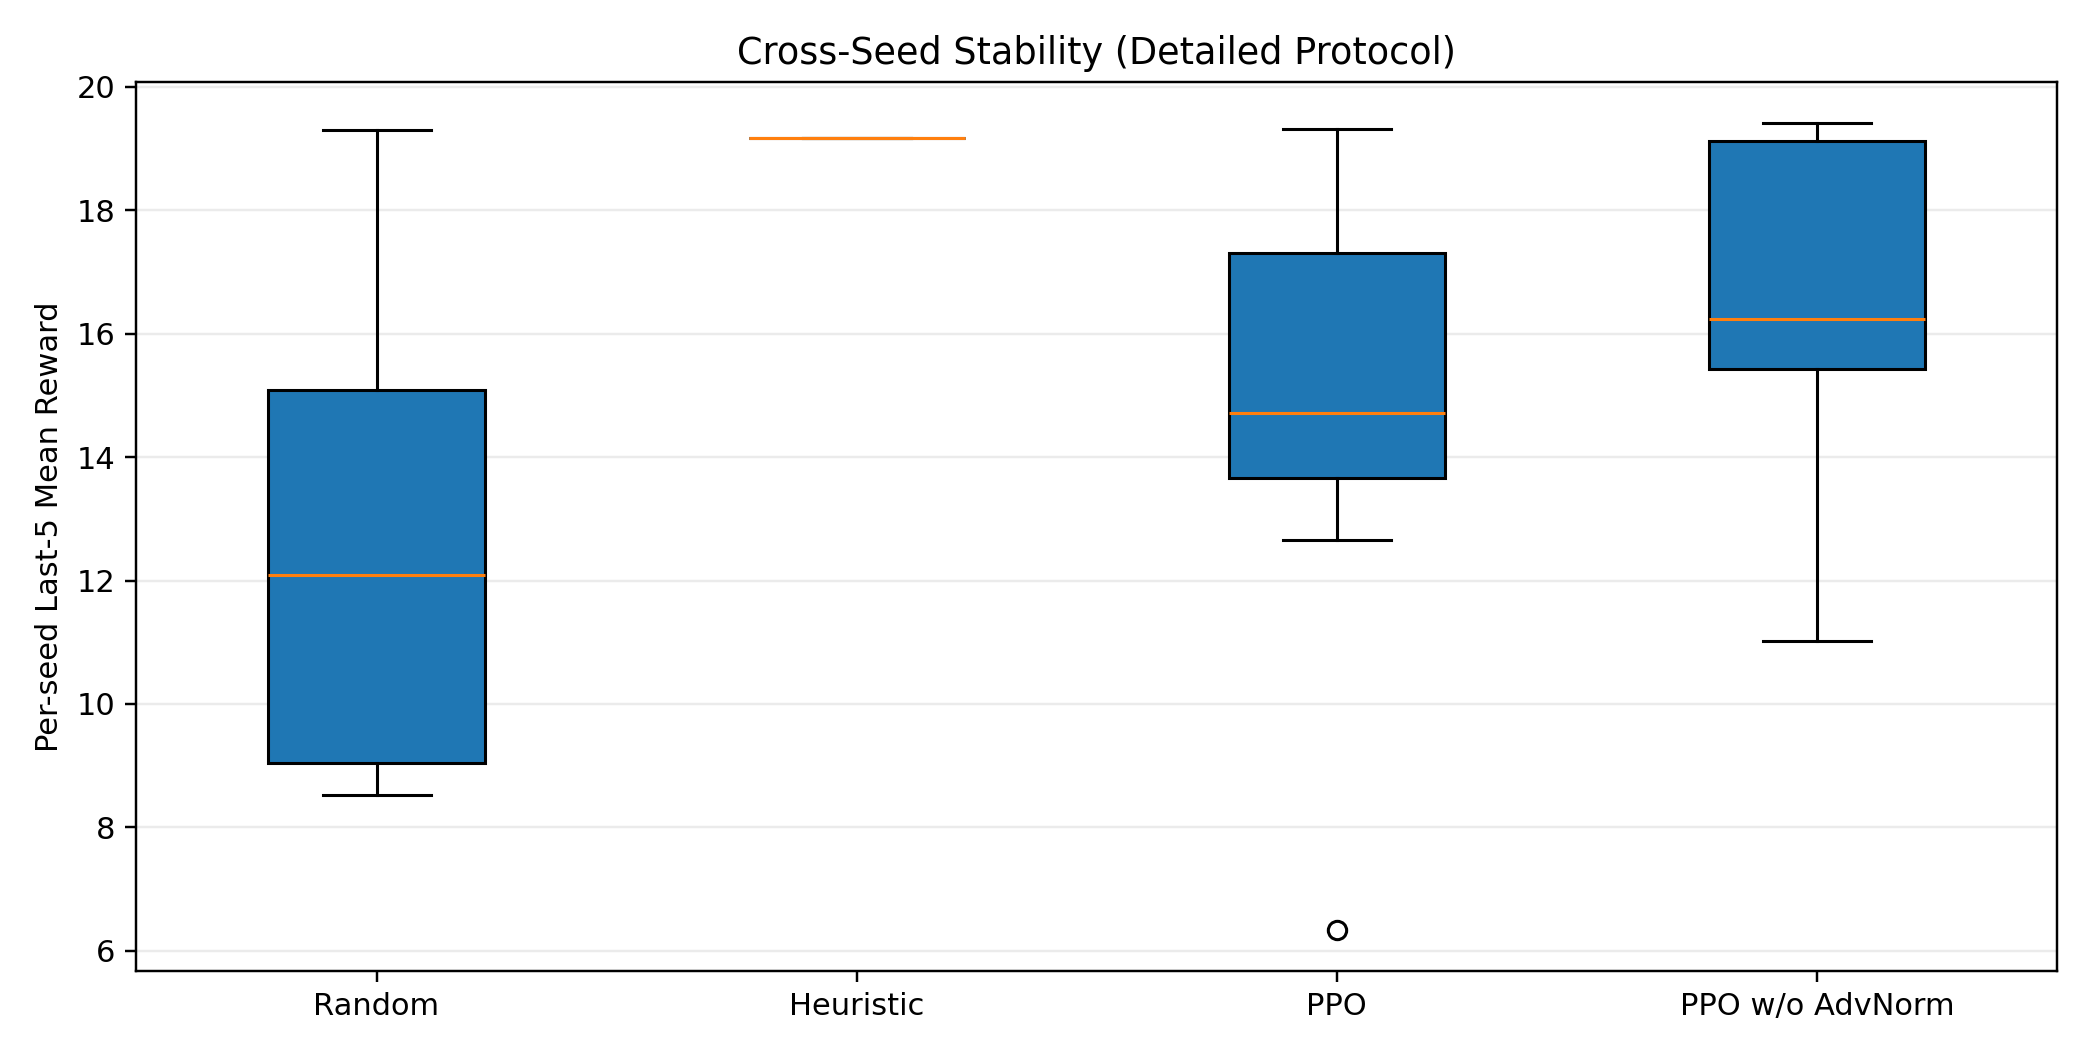
\includegraphics[width=0.86\linewidth]{figures/seed_stability_boxplot.png}
\caption{Distribution of per-seed final-window reward.}
\label{fig:seed-boxplot}
\end{figure}

Confidence intervals and box plots together show that heuristic policy is not only stronger in average performance, but also substantially tighter in variance. PPO spreads are broad, especially in tails, suggesting sensitivity to initialization and stochastic transition realizations.

\begin{figure}[H]
\centering
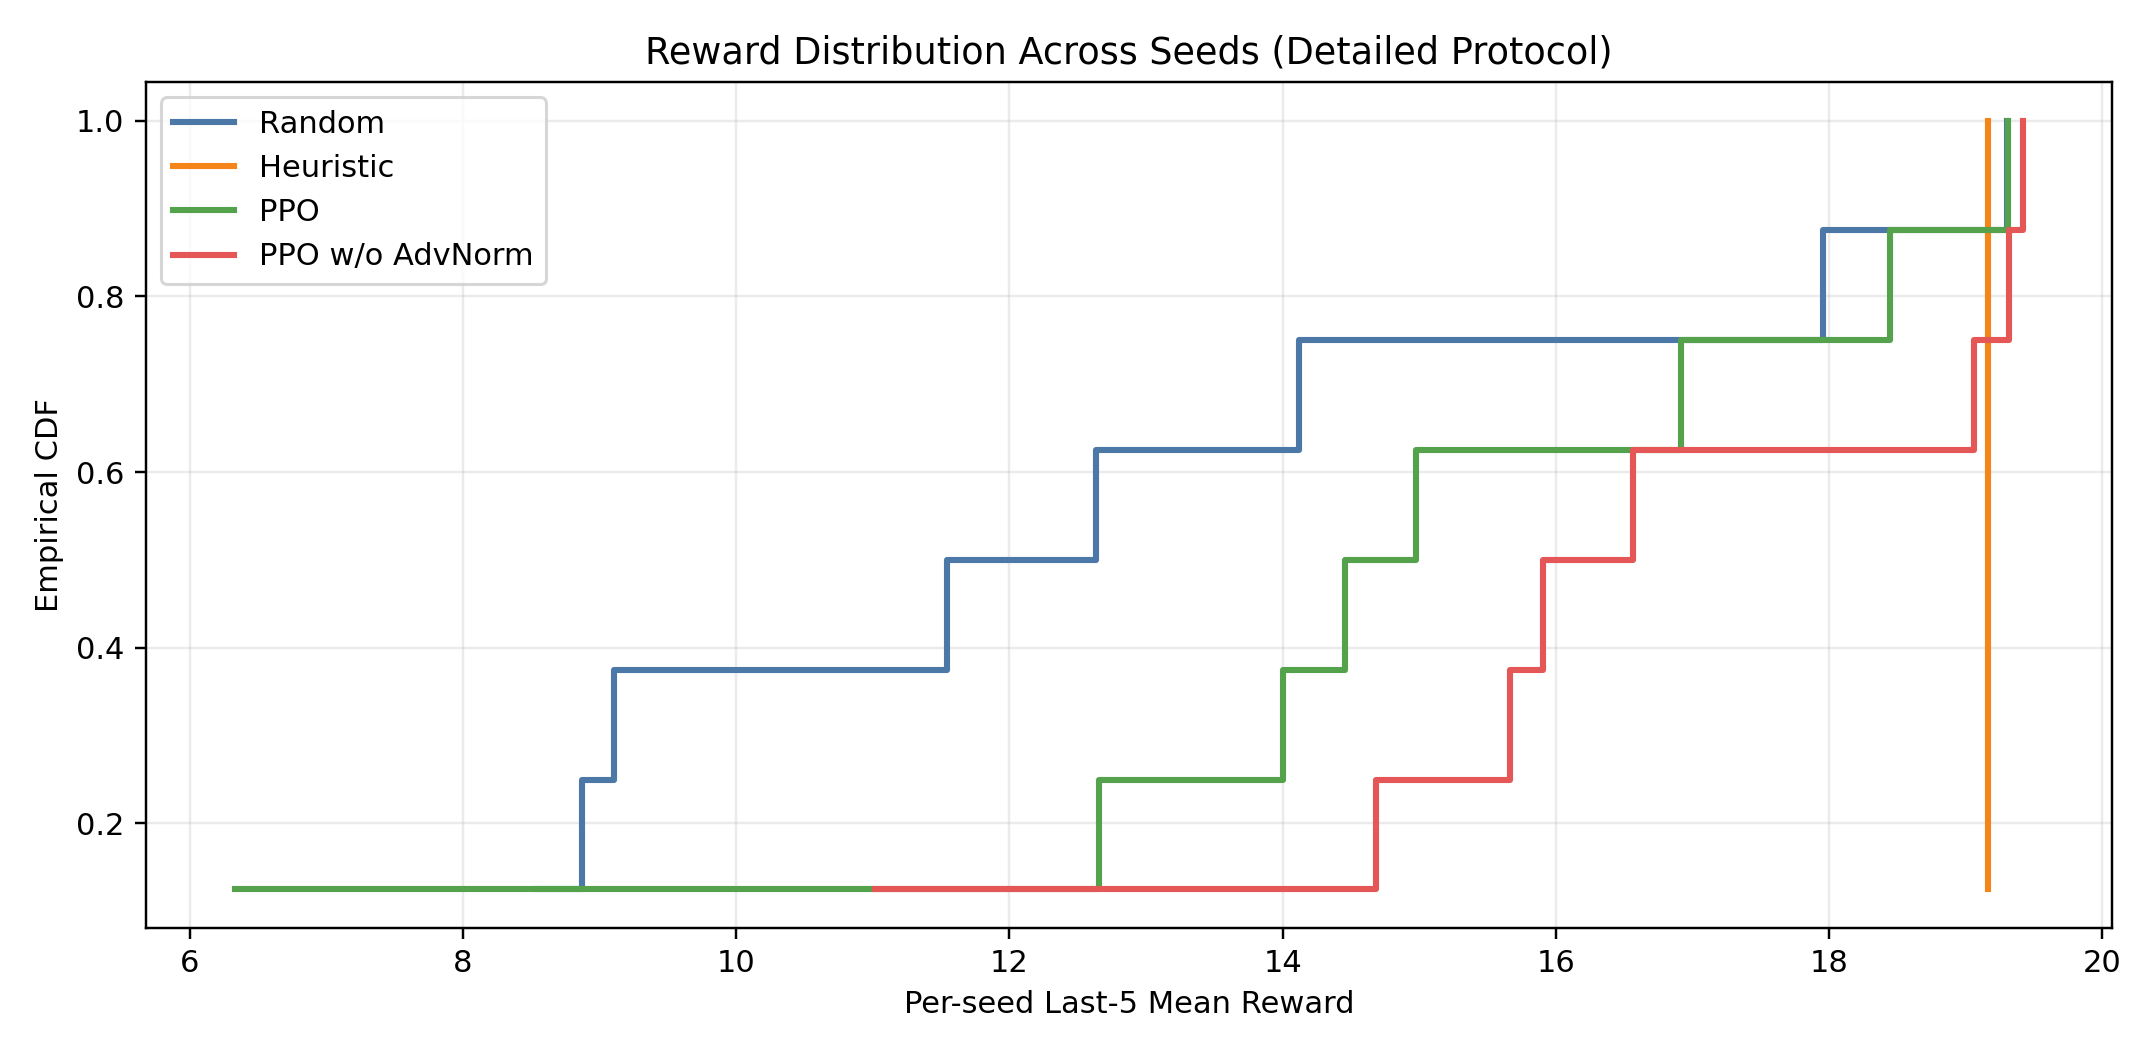
\includegraphics[width=0.86\linewidth]{figures/reward_ecdf.png}
\caption{Empirical CDF of per-seed reward for the detailed 60-episode protocol.}
\label{fig:reward-ecdf}
\end{figure}

\begin{figure}[H]
\centering
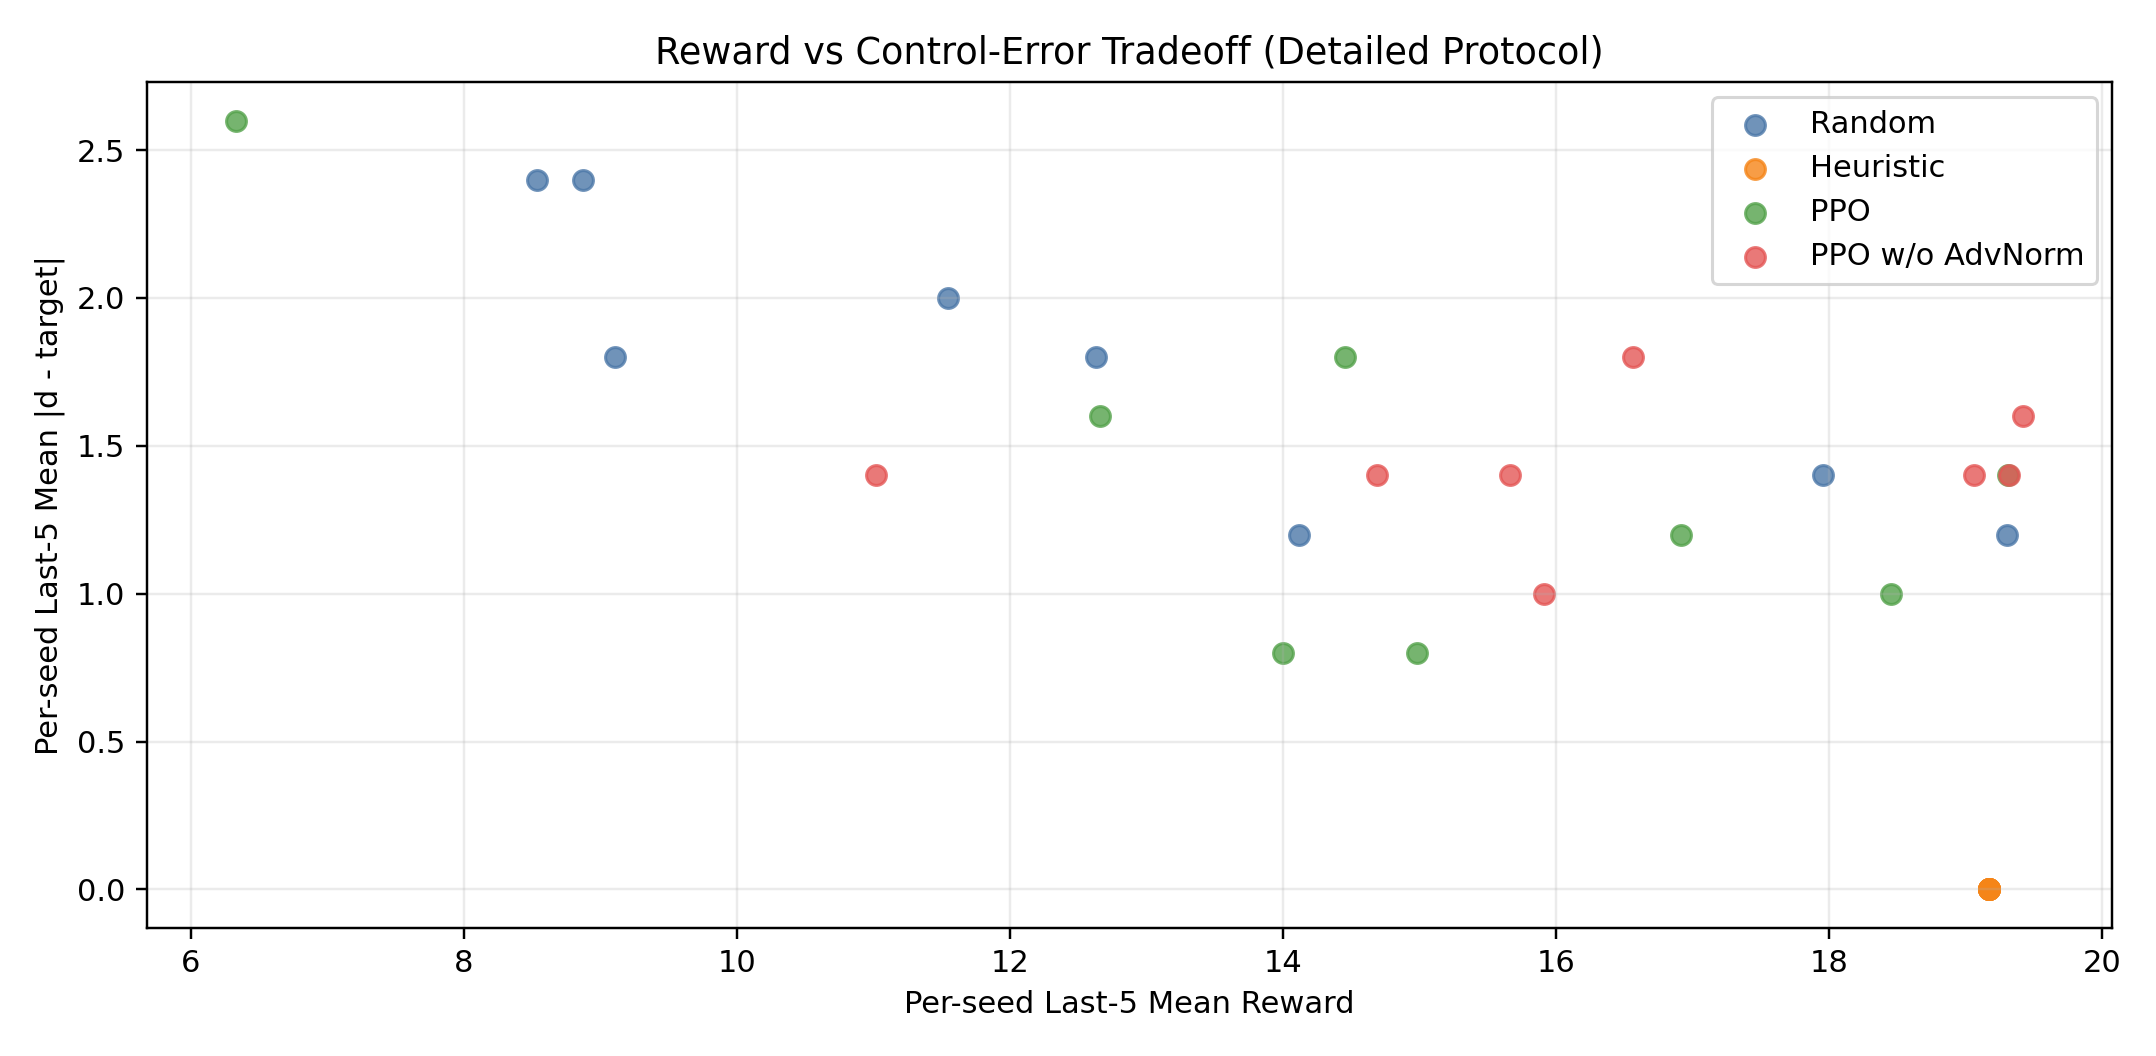
\includegraphics[width=0.86\linewidth]{figures/reward_error_tradeoff.png}
\caption{Per-seed tradeoff between reward and target-tracking error.}
\label{fig:reward-error-tradeoff}
\end{figure}

\begin{figure}[H]
\centering
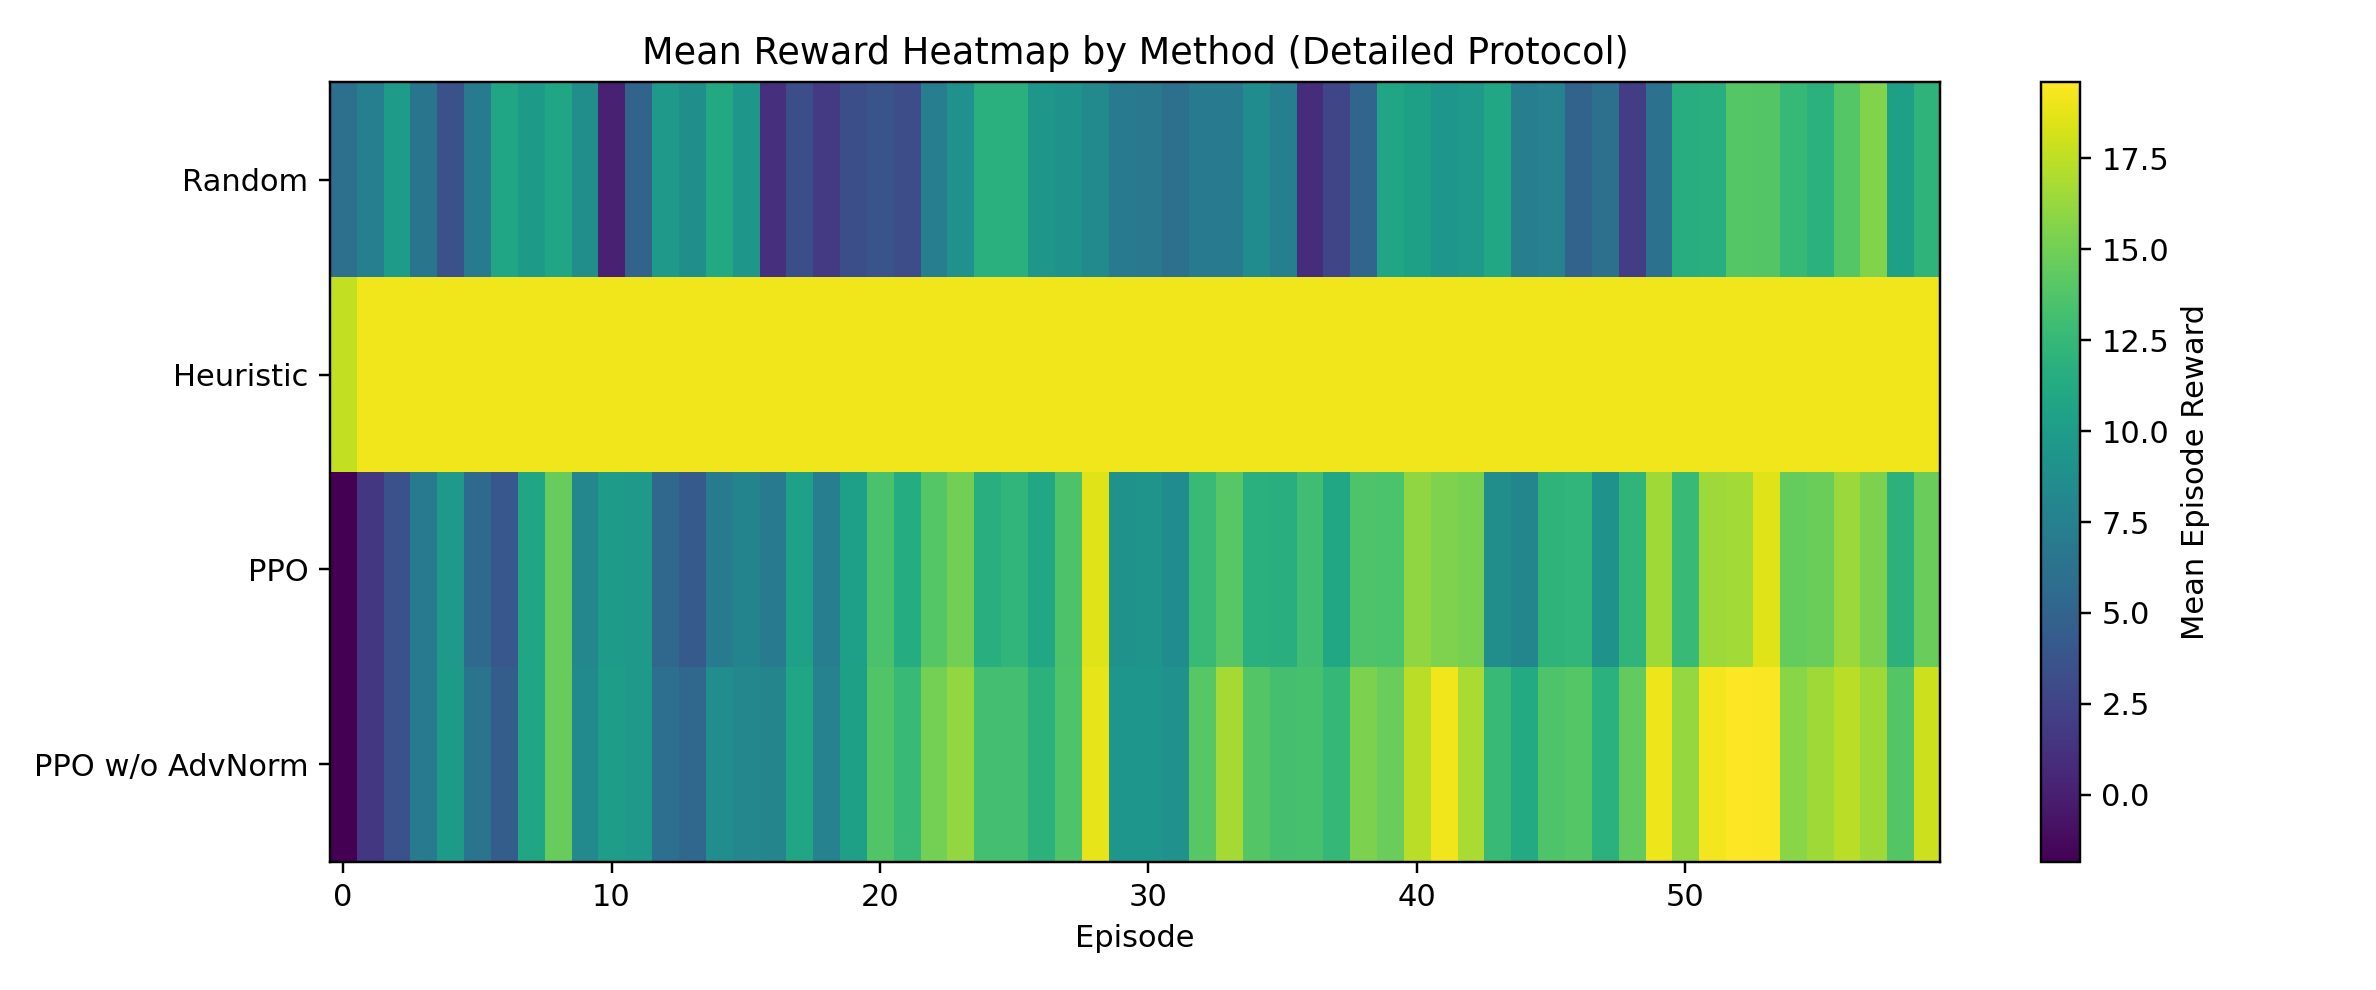
\includegraphics[width=0.92\linewidth]{figures/reward_heatmap.png}
\caption{Episode-method reward heatmap from detailed trajectory data.}
\label{fig:reward-heatmap}
\end{figure}

\begin{figure}[H]
\centering
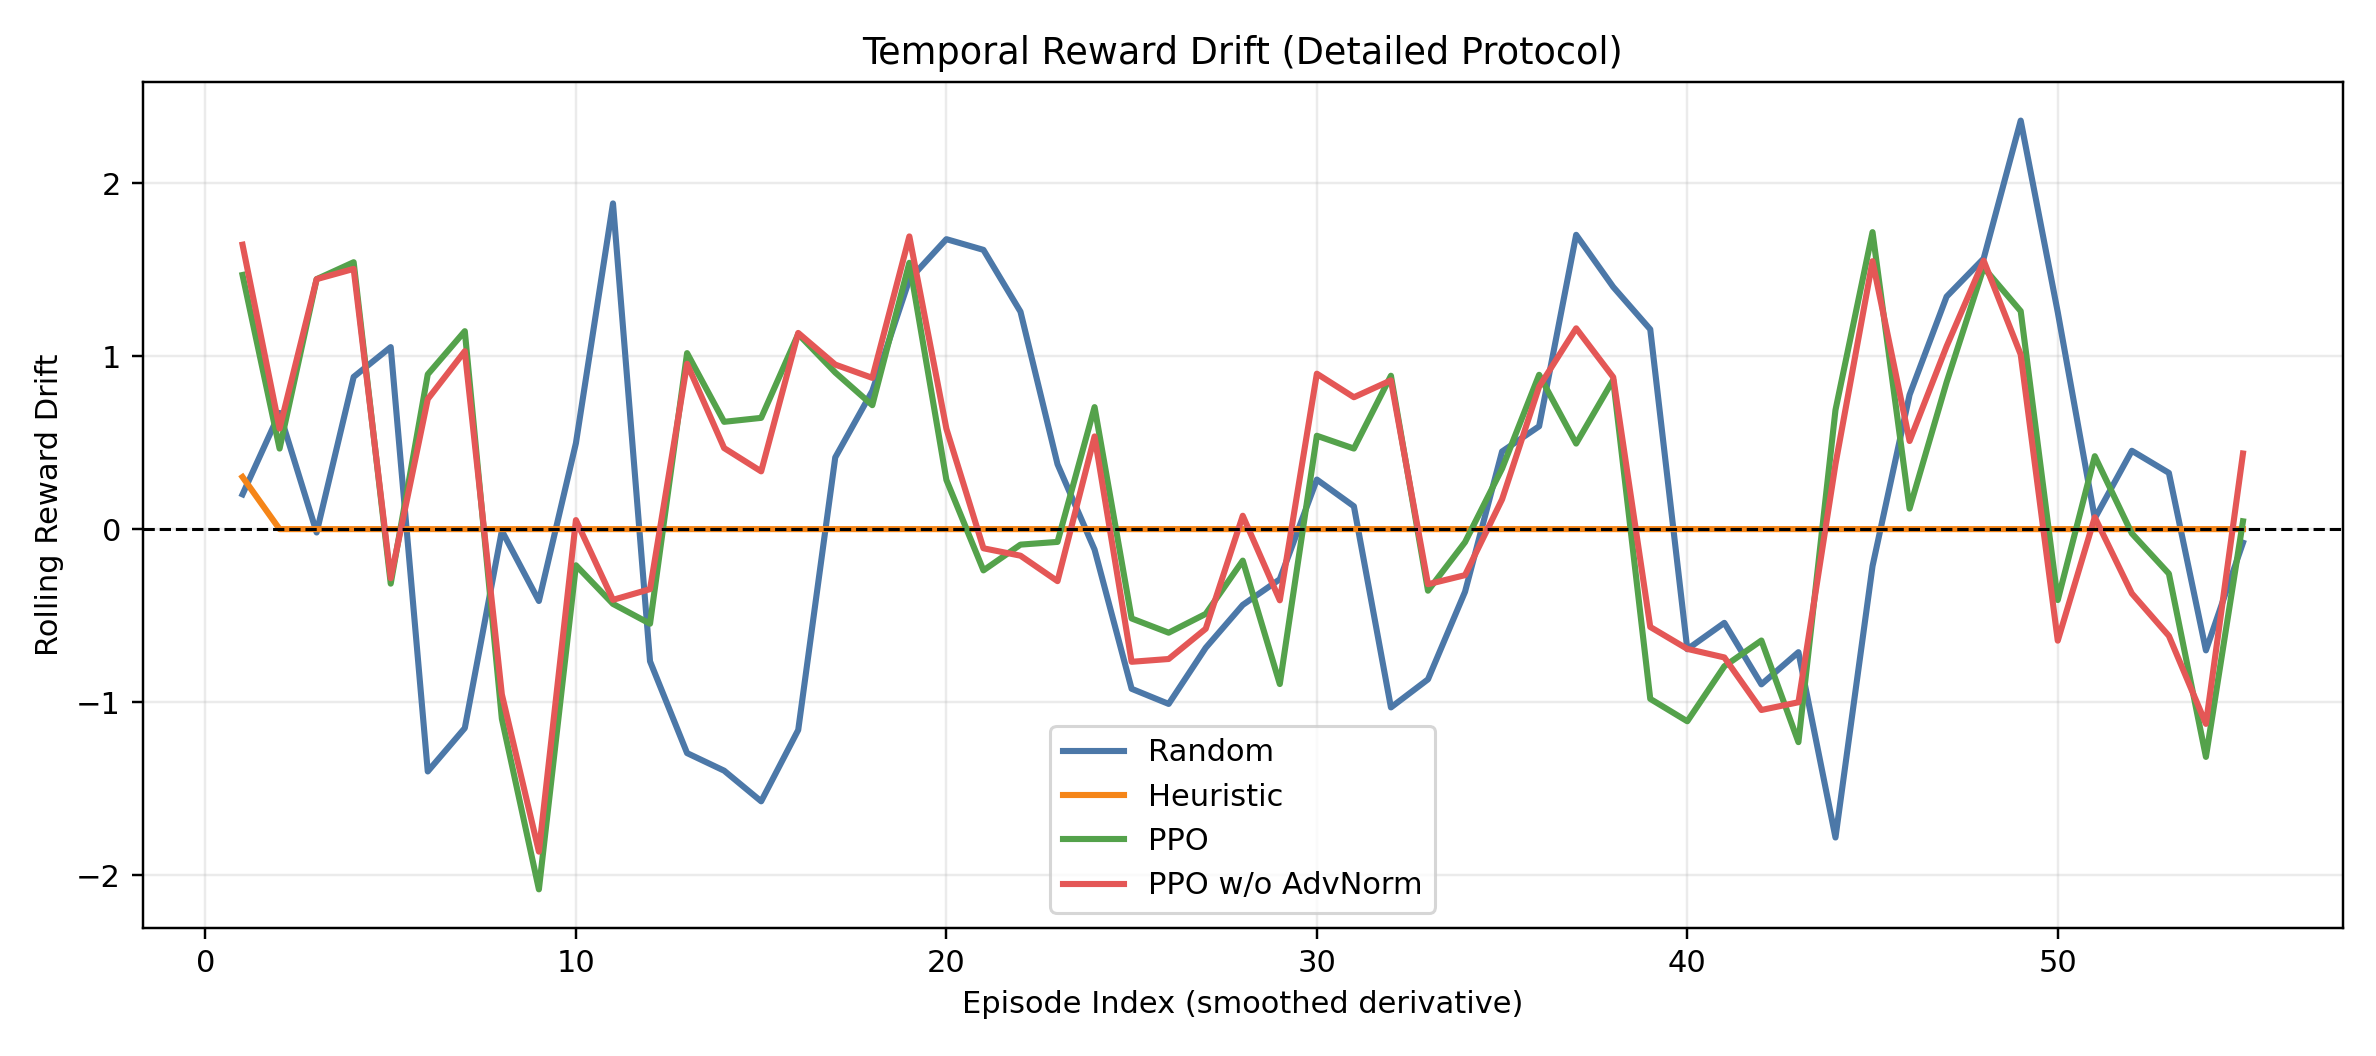
\includegraphics[width=0.90\linewidth]{figures/reward_drift.png}
\caption{Rolling temporal drift of mean reward (smoothed derivative) across episodes.}
\label{fig:reward-drift}
\end{figure}

\begin{figure}[H]
\centering
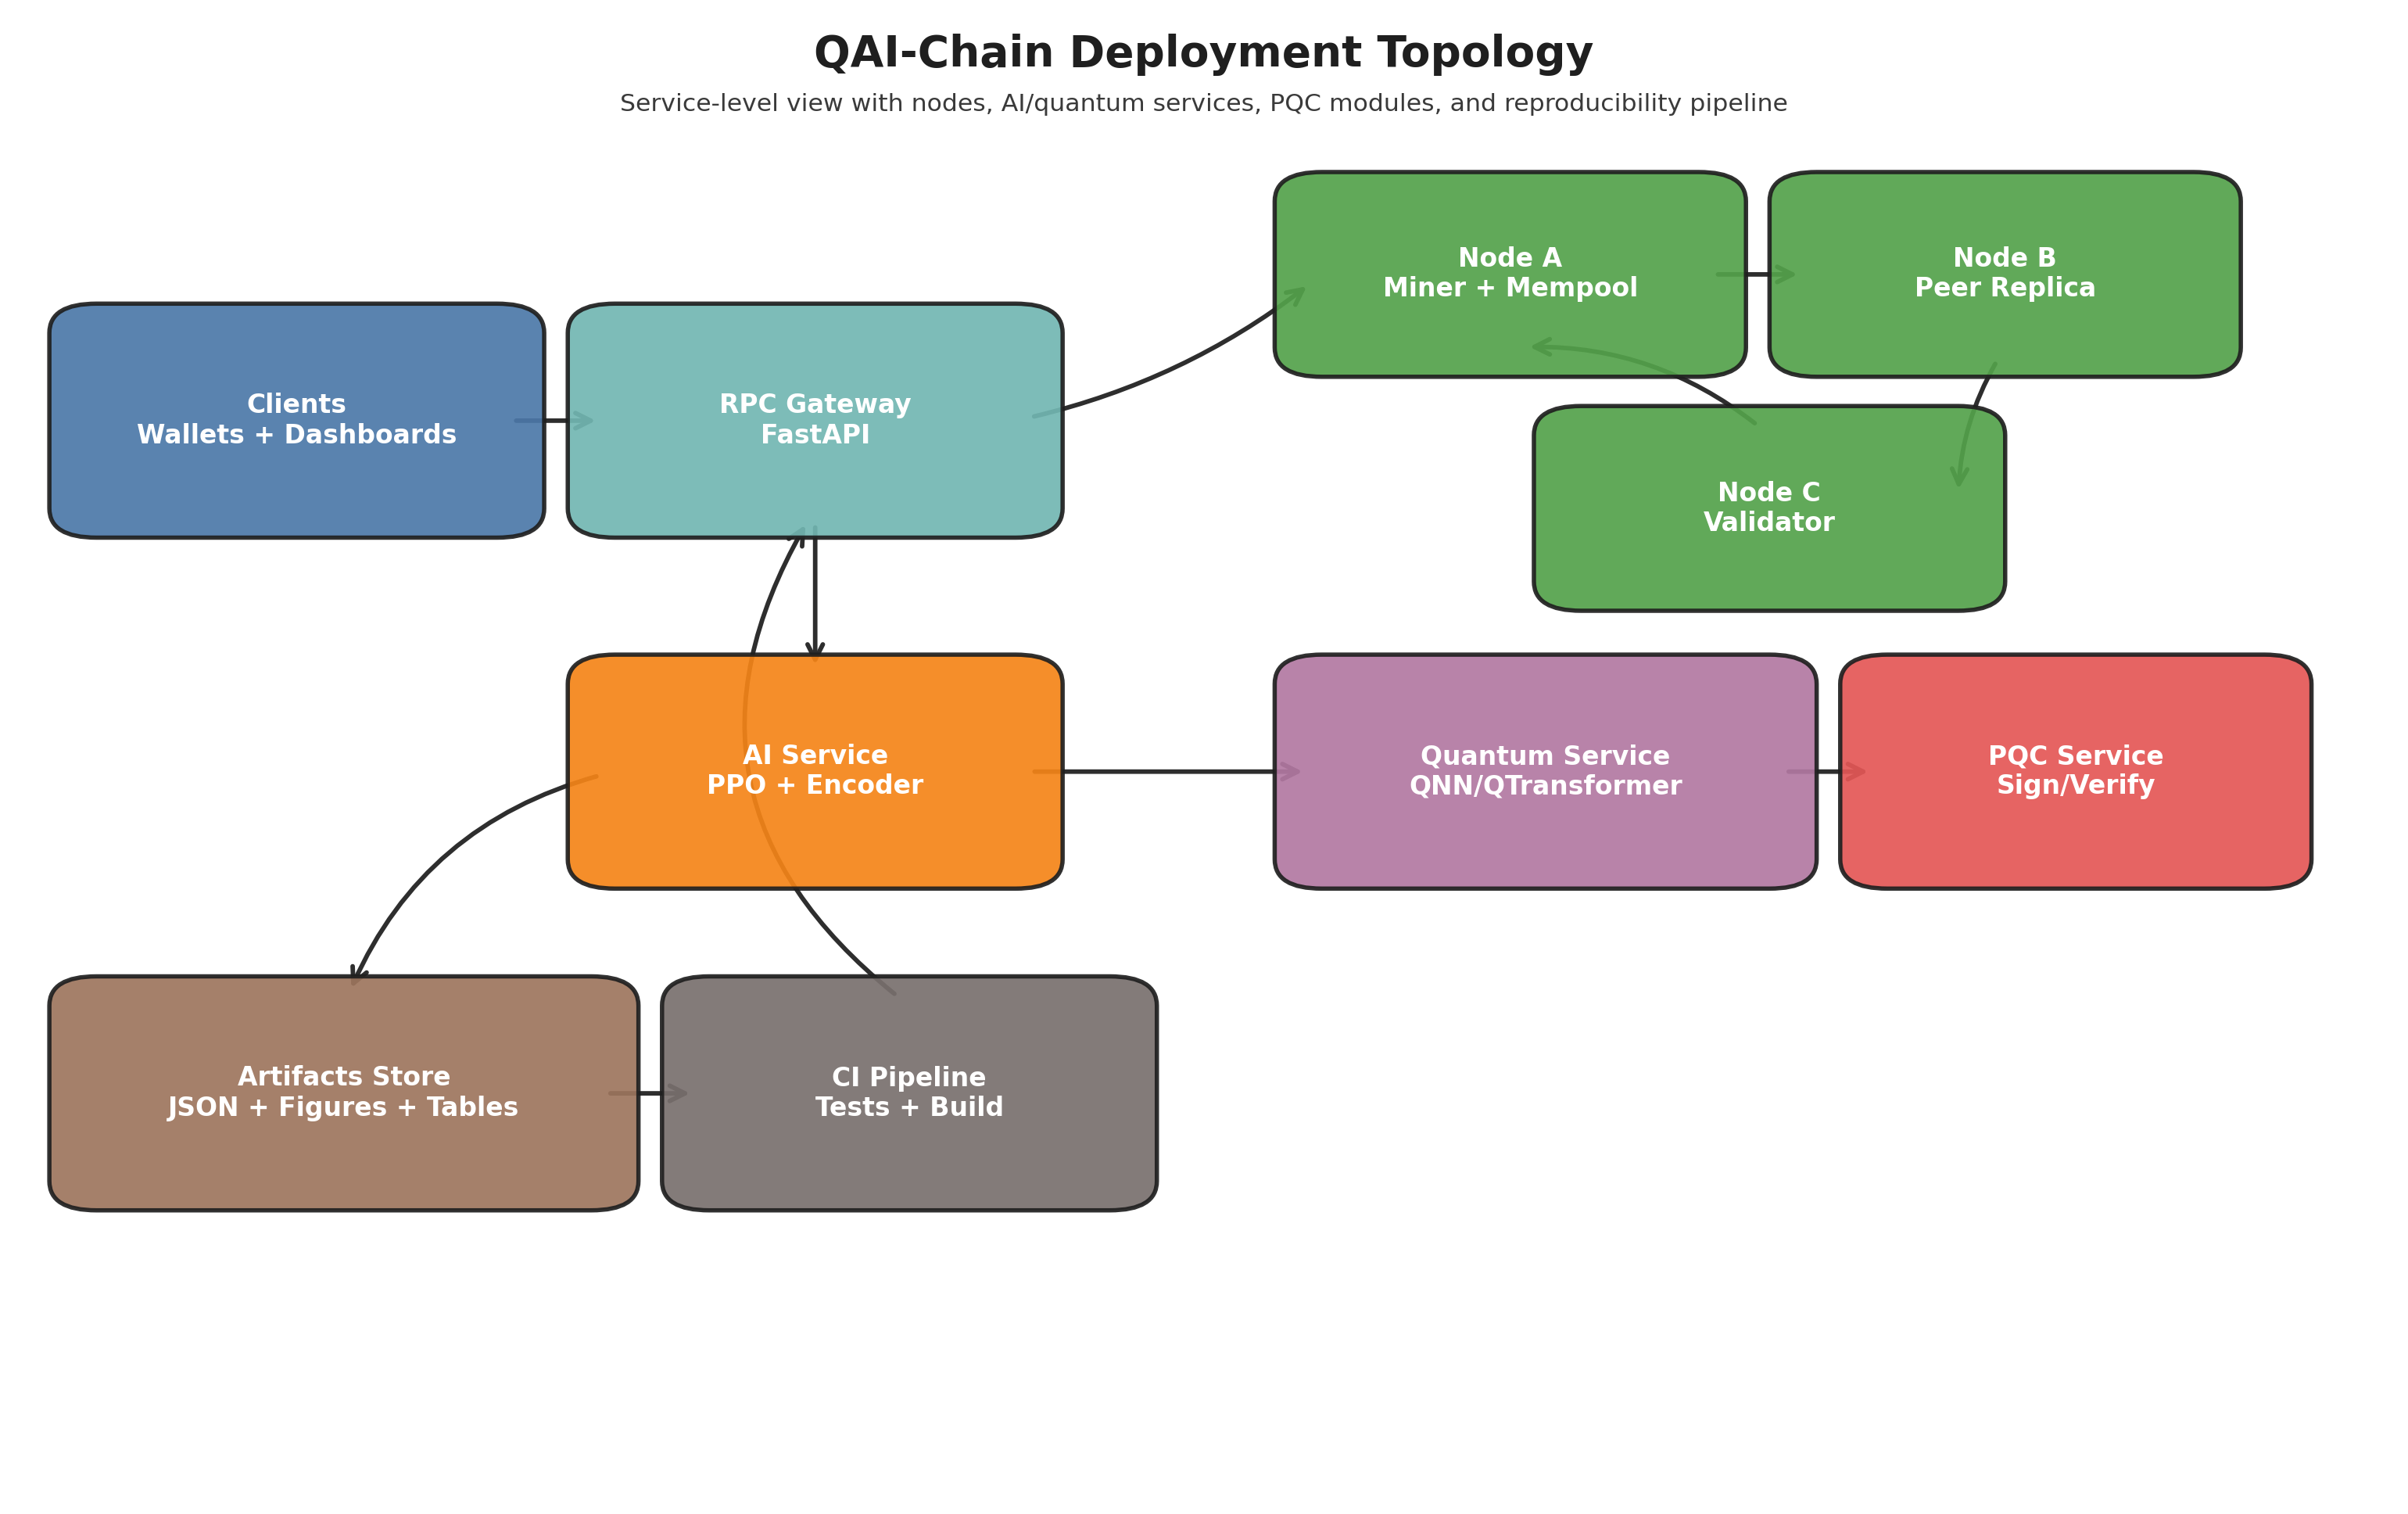
\includegraphics[width=0.95\linewidth]{figures/deployment_topology.png}
\caption{Deployment topology view: RPC gateway, multi-node blockchain layer, AI/quantum services, PQC, and CI-artifact loop.}
\label{fig:deployment-topology}
\end{figure}

\begin{figure}[H]
\centering
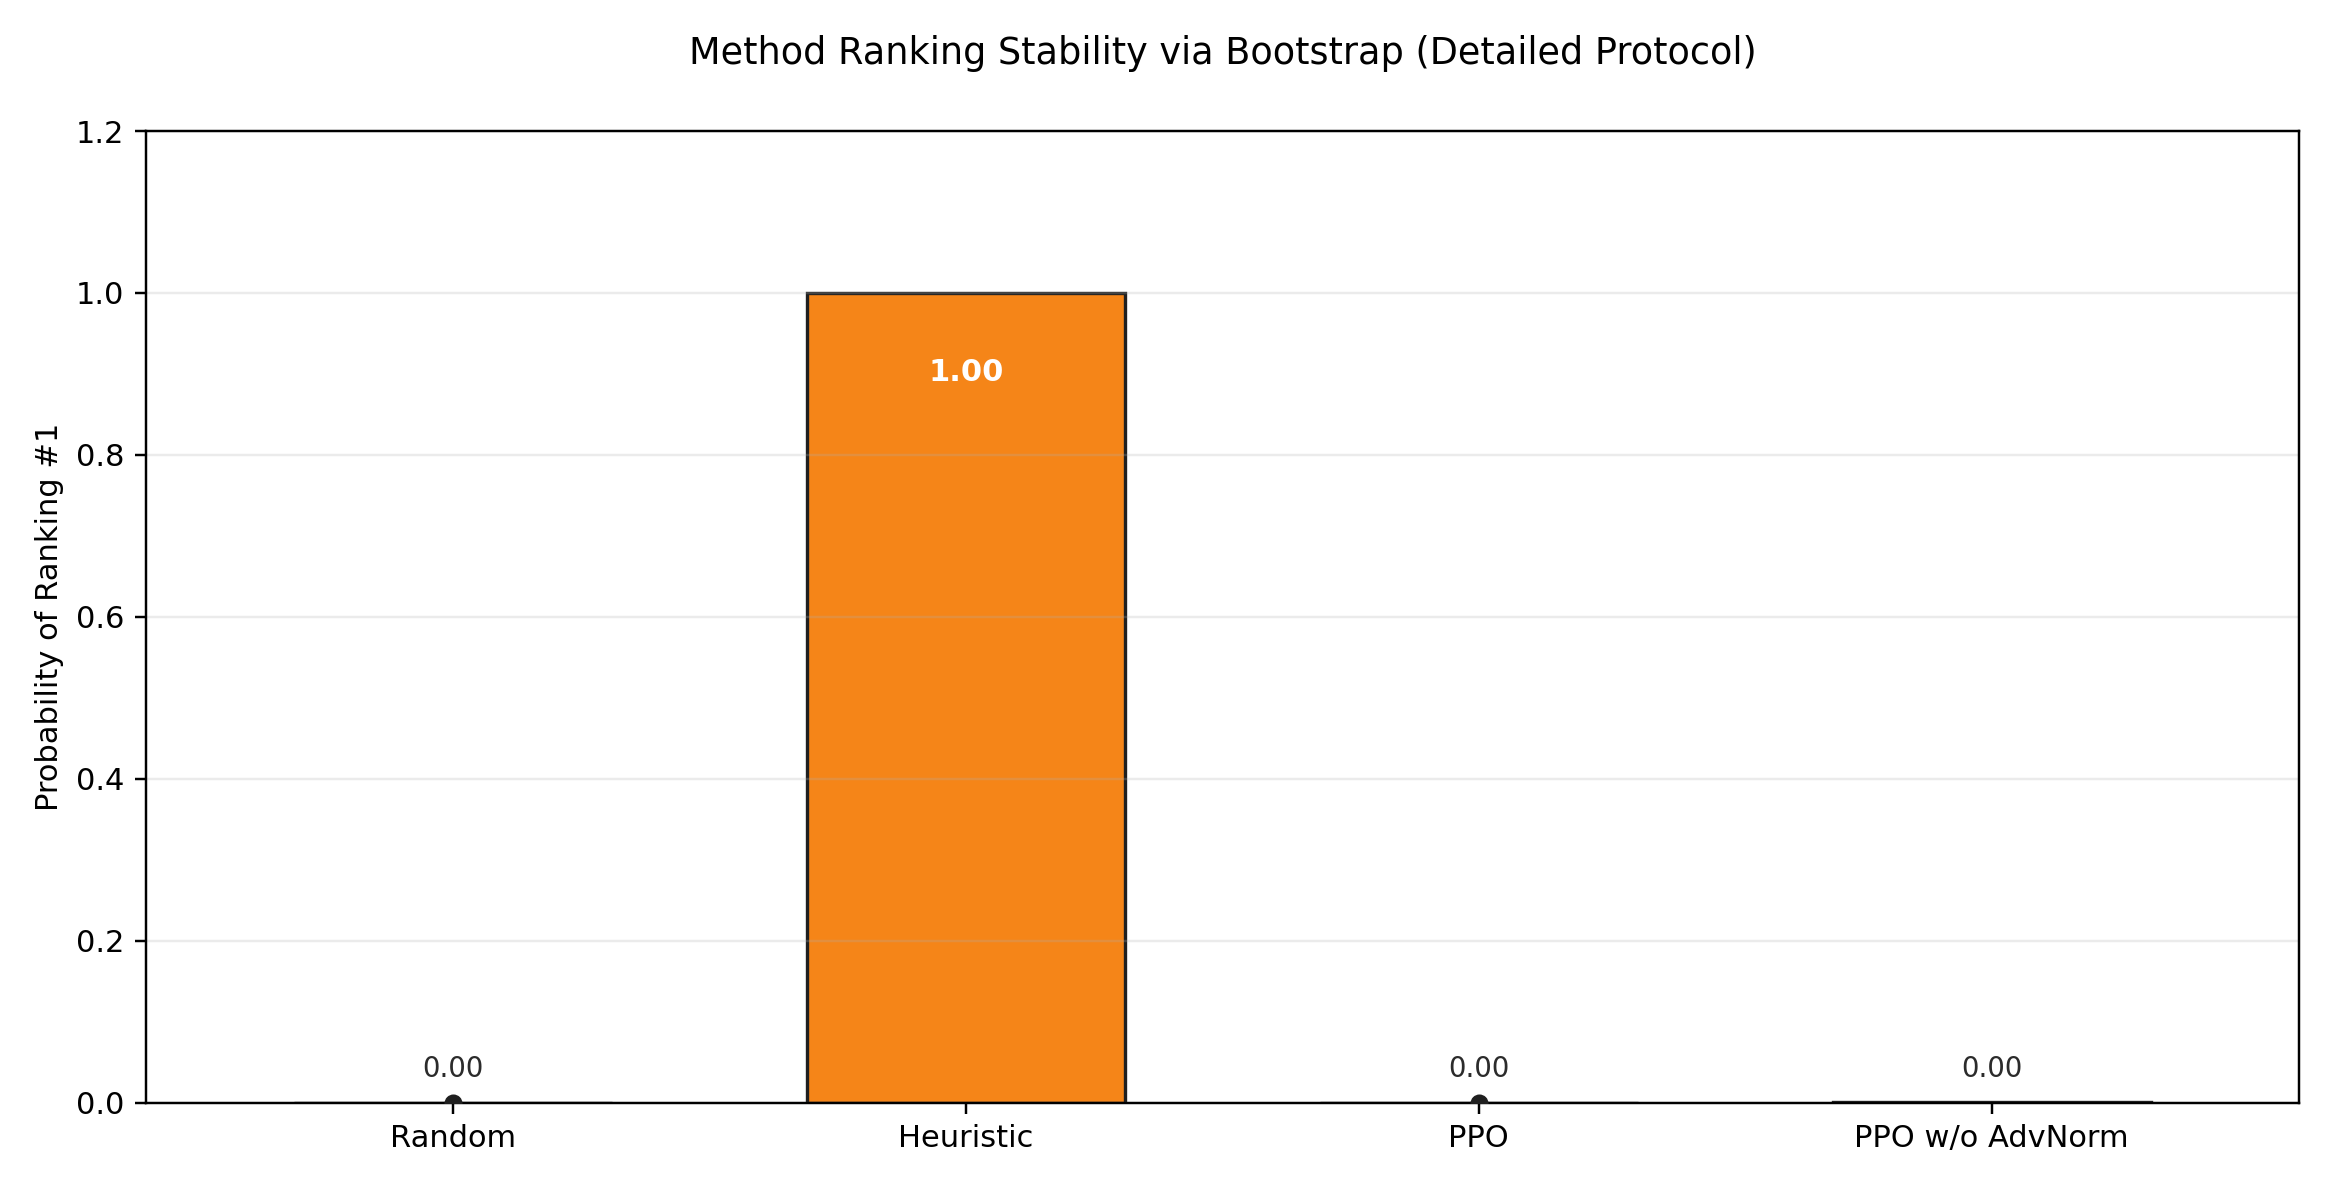
\includegraphics[width=0.86\linewidth]{figures/rank_stability_bootstrap.png}
\caption{Bootstrap ranking stability: probability that each method ranks first by mean reward under resampling.}
\label{fig:rank-stability}
\end{figure}

The ECDF and tradeoff views complement means and confidence intervals reported in Section~\ref{sec:results}: they expose tail behavior and reward-calibration structure at seed level. The heatmap reveals temporal regimes where PPO variants transition from underperforming to competitive in subsets of episodes, but still fail to achieve heuristic-level consistency. The drift plot adds a trend-signal perspective, showing where each method gains or loses momentum over training time. The deployment topology figure clarifies how empirical results map to a deployable service layout. Finally, the bootstrap ranking-stability view reports how often each method is top-ranked under resampling, providing a compact robustness check for comparative claims.

\begin{figure}[H]
\centering
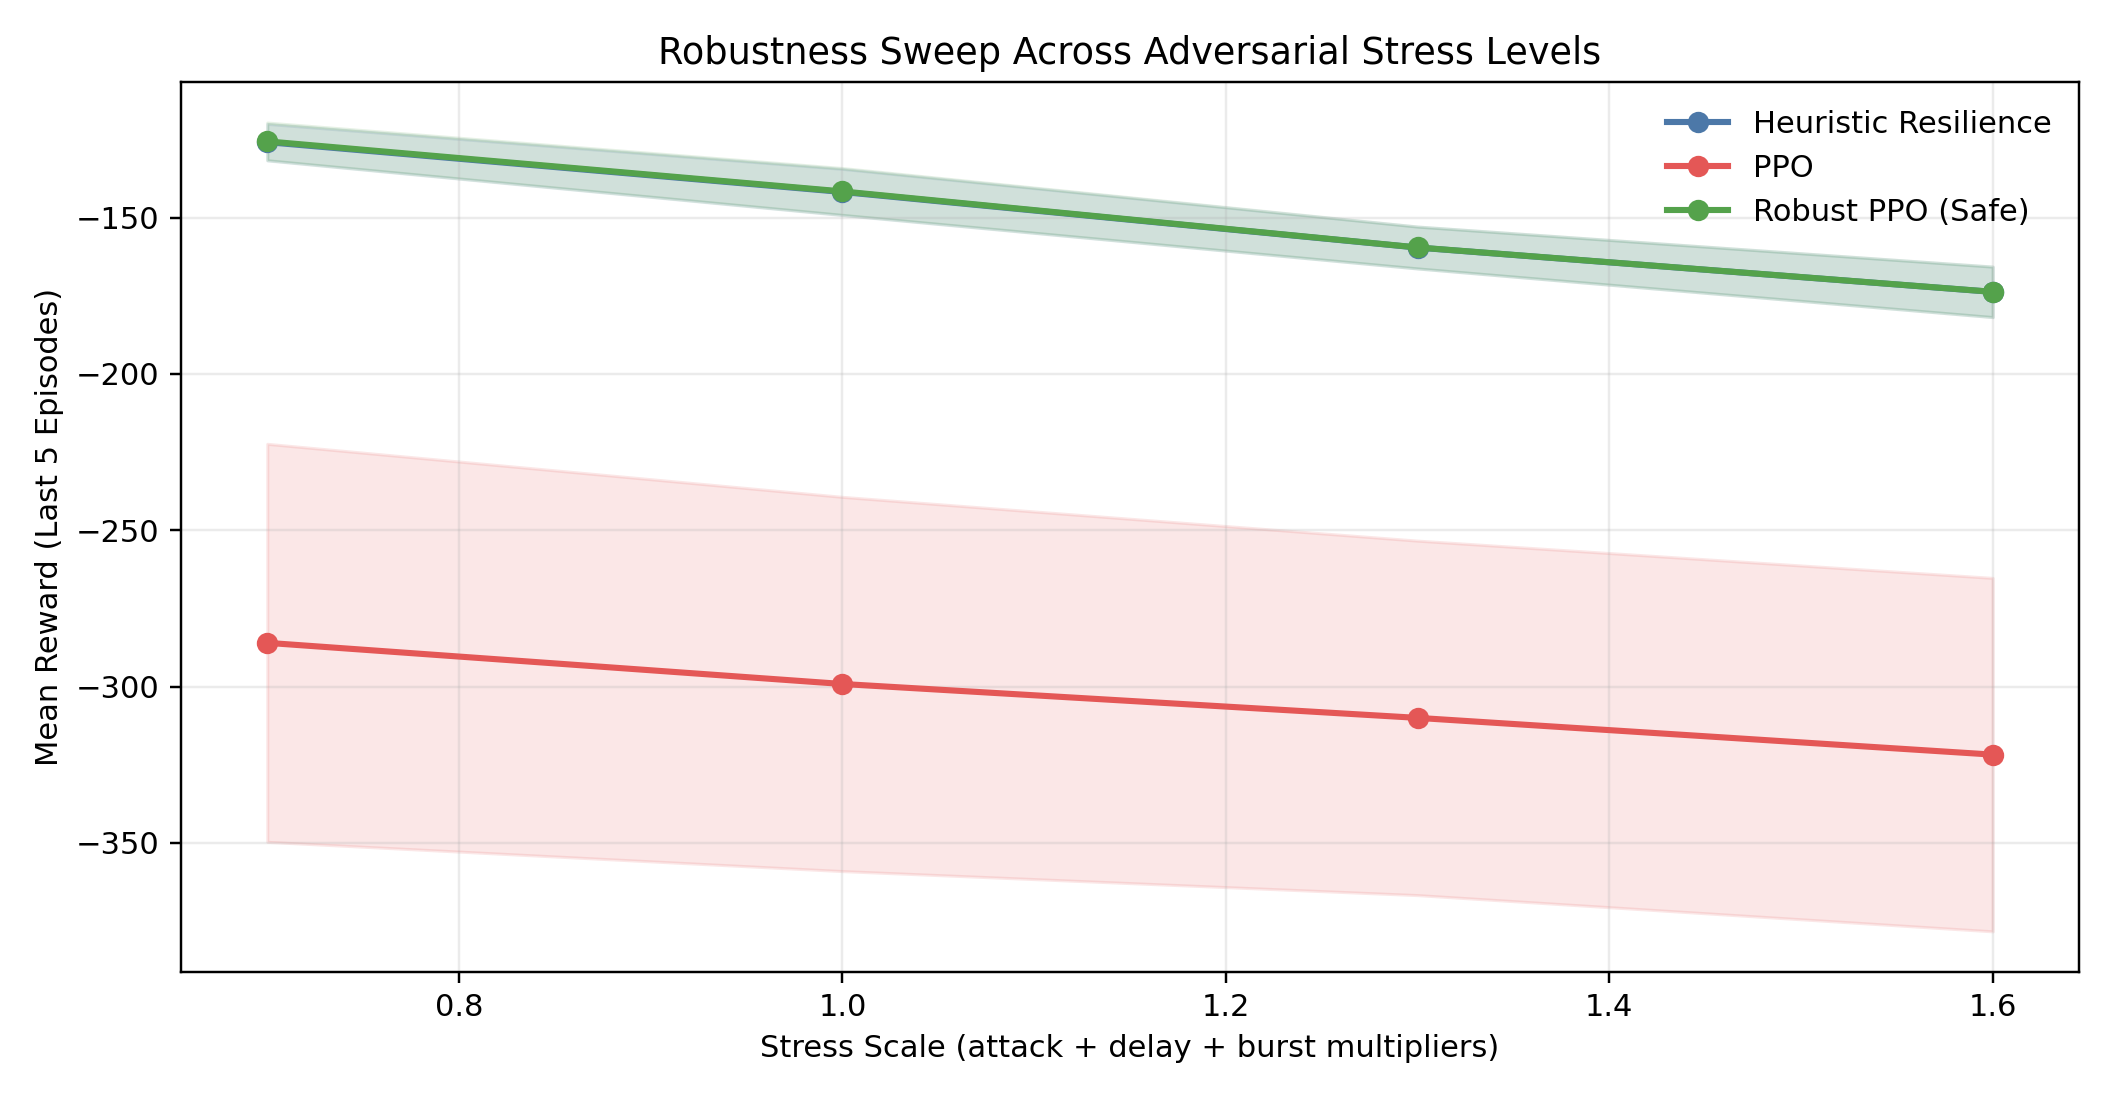
\includegraphics[width=0.88\linewidth]{figures/adversarial_stress_sweep.png}
\caption{Stress sweep over adversarial intensity: Robust PPO remains consistently above vanilla PPO and near/above the resilience heuristic across regimes.}
\label{fig:adversarial-stress-sweep}
\end{figure}

This stress-sweep result improves external validity of the adversarial claim: Robust PPO is not tuned for a single disturbance point, but remains competitive under progressively harsher combinations of attack probability, delay noise, and burst pressure.

\subsection{Complexity Regime Sweep}

To address the limitation of low-complexity governance tasks, we introduce a regime-sweep benchmark where hidden control regimes switch more frequently as complexity increases. This creates decision surfaces that are harder for fixed-rule heuristics to track.

\begin{table}[H]
\centering
\small
\setlength{\tabcolsep}{6pt}
\begin{tabular}{lcccc}
\toprule
Method & C=0.6 & C=1.0 & C=1.4 & C=1.8 \\
\midrule
Heuristic Resilience & -416.32 $\pm$ 39.34 & -415.42 $\pm$ 40.21 & -416.79 $\pm$ 43.17 & -428.83 $\pm$ 24.27 \\
PPO & -409.65 $\pm$ 48.09 & -388.53 $\pm$ 42.05 & -396.19 $\pm$ 33.73 & -392.76 $\pm$ 41.36 \\
Robust PPO (Safe) & -397.56 $\pm$ 32.59 & -400.12 $\pm$ 33.48 & -374.87 $\pm$ 30.57 & -391.01 $\pm$ 36.36 \\
\bottomrule
\end{tabular}

\caption{Complexity sweep summary across regime-switch intensities.}
\label{tab:complexity-regime}
\end{table}

\begin{figure}[H]
\centering
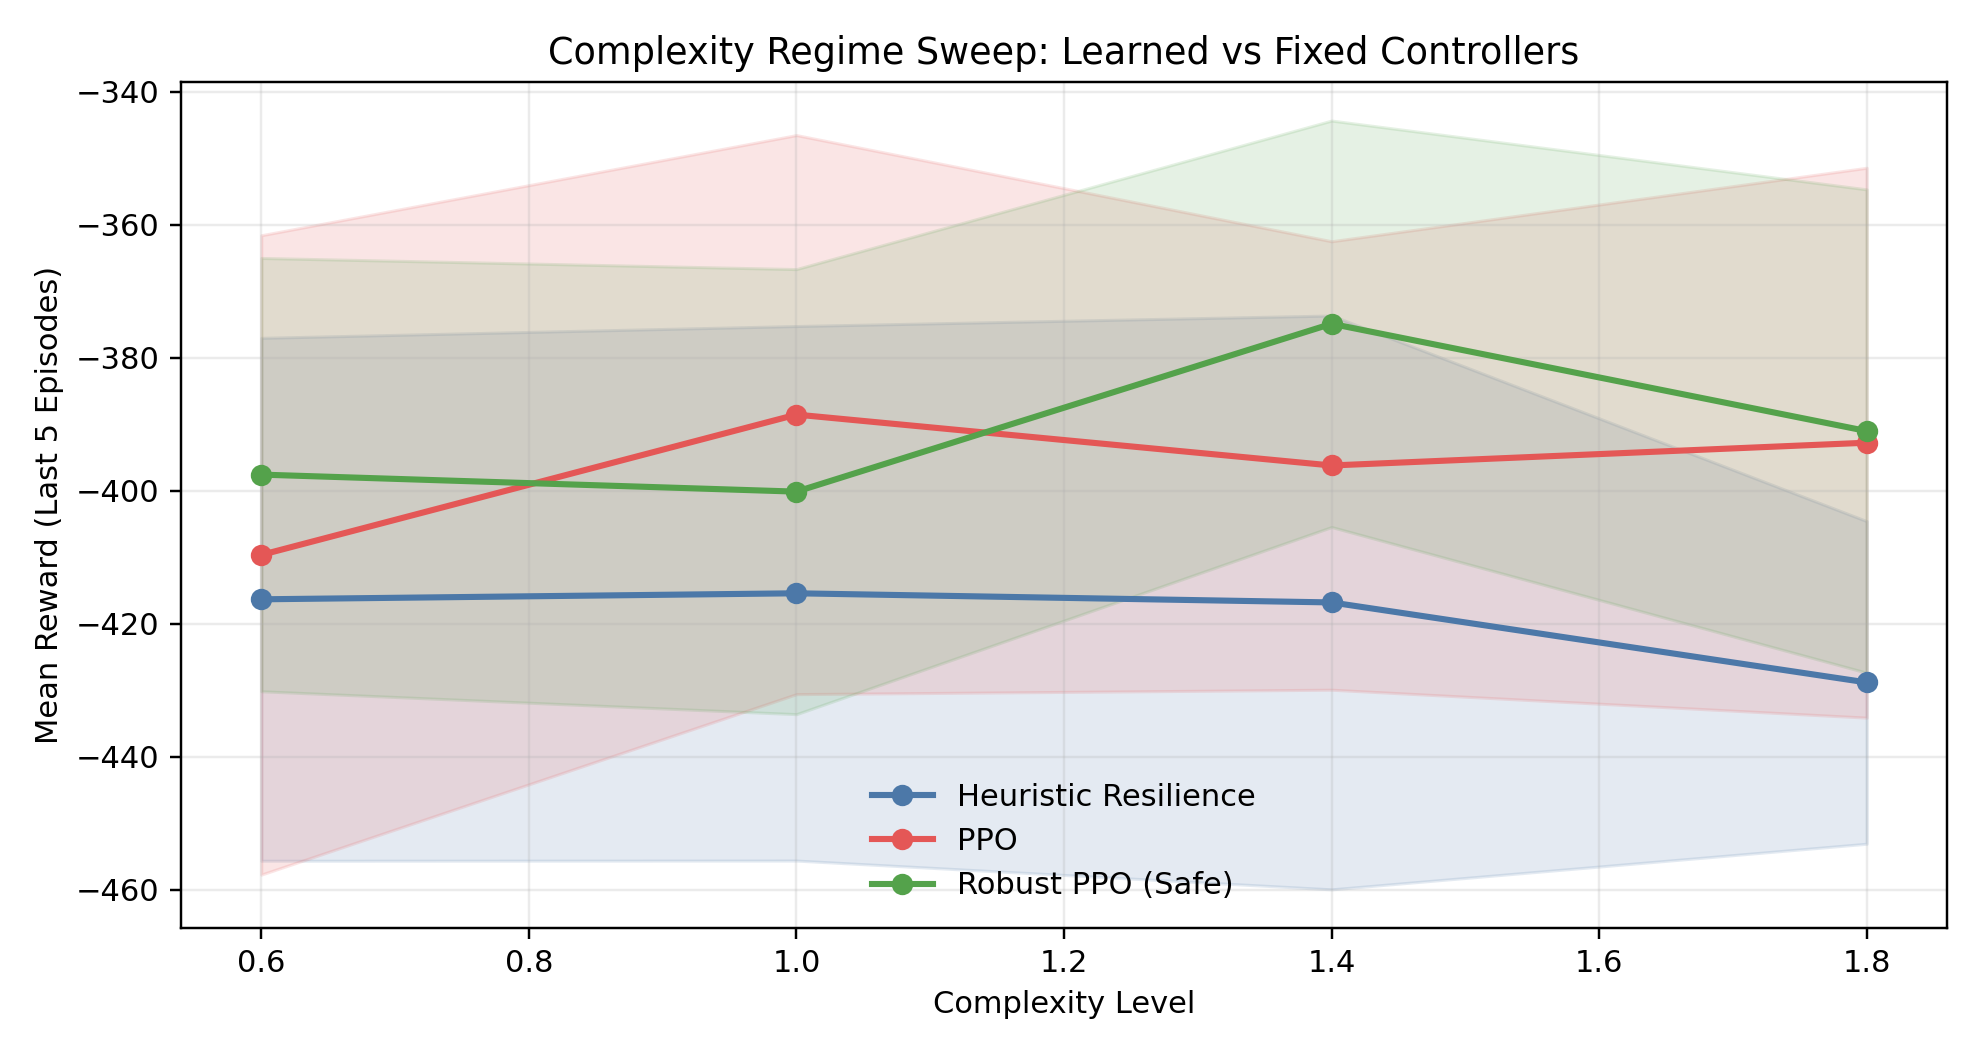
\includegraphics[width=0.88\linewidth]{figures/complexity_regime_sweep.png}
\caption{Complexity-regime sweep: learned controllers improve reward under increasing regime-switch difficulty; Robust PPO remains closer to heuristic calibration than vanilla PPO.}
\label{fig:complexity-regime}
\end{figure}

As complexity grows, fixed heuristics lose reward efficiency relative to learned policies. In mid complexity ($C=1.0$), PPO still has a reward edge. In higher complexity ($C=1.4$ and $C=1.8$), tuned Robust PPO overtakes PPO on reward while keeping lower target-tracking error. The practical interpretation is straightforward: when regime switches accelerate, uncertainty-aware control and risk shaping become performance features, not just safety add-ons.

\subsection{Trajectory and Seed Tables}

\begin{table}[H]
\centering
\begin{tabular}{lccccc}
\toprule
Method & Ep1 & Ep10 & Ep20 & Ep40 & Ep60 \\
\midrule
Random & 6.10 & 8.73 & 3.35 & 10.79 & 12.13 \\
Heuristic & 17.66 & 19.17 & 19.17 & 19.17 & 19.17 \\
PPO & -1.84 & 8.07 & 10.24 & 13.53 & 14.74 \\
PPO w/o AdvNorm & -1.84 & 8.38 & 10.31 & 14.73 & 17.98 \\
\bottomrule
\end{tabular}

\caption{Reward trajectory snapshots at selected episode indices for the 60-episode suite.}
\label{tab:trajectory-summary}
\end{table}

\begin{table}[H]
\centering
\begin{tabular}{lccc}
\toprule
Method & Mean Final Difficulty & Std Final Difficulty & Mean $|d-d_t|$ \\
\midrule
Random & 4.00 & 1.80 & 1.75 \\
Heuristic & 3.00 & 0.00 & 0.00 \\
PPO & 2.75 & 1.20 & 1.00 \\
PPO w/o AdvNorm & 1.75 & 0.66 & 1.25 \\
\bottomrule
\end{tabular}

\caption{Final-difficulty behavior and target tracking statistics in the detailed suite.}
\label{tab:difficulty-summary}
\end{table}

\begin{table}[H]
\centering
\begin{tabular}{lcccc}
\toprule
Seed & Random & Heuristic & PPO & PPO w/o AdvNorm \\
\midrule
3 & 11.54 & 19.17 & 14.46 & 16.56 \\
7 & 9.10 & 19.17 & 19.31 & 19.42 \\
11 & 12.63 & 19.17 & 6.33 & 11.02 \\
17 & 8.87 & 19.17 & 12.66 & 14.69 \\
21 & 17.96 & 19.17 & 18.45 & 19.32 \\
42 & 14.12 & 19.17 & 14.98 & 15.91 \\
84 & 8.53 & 19.17 & 16.92 & 19.06 \\
126 & 19.30 & 19.17 & 14.00 & 15.66 \\
\bottomrule
\end{tabular}

\caption{Per-seed mean reward over last five episodes.}
\label{tab:seed-scores}
\end{table}

The seed table shows a practical pattern: some seeds produce PPO behavior near heuristic performance, while others regress toward random-like outcomes. This motivates robust policy selection mechanisms (for example, ensemble checkpoints, uncertainty-aware fallback policies, or adaptive safety constraints) before deployment.

\FloatBarrier
